%
% $Id: paper.tex,v 1.4 2005/04/04 10:38:07 kiniry Exp $
%

\documentclass{entcs}

% \usepackage{latex8}
\usepackage{entcsmacro}
\usepackage{times}
\usepackage{ifpdf}
% \usepackage{a4wide}

\ifpdf
\usepackage[pdftex]{graphicx}
\else
\usepackage{graphicx}
\fi

% \usepackage{html}
% \usepackage{url}
\usepackage{xspace}
%\usepackage{doublespace}
\usepackage{tabularx}
\usepackage{epsfig}
% \usepackage{amsmath}
% \usepackage{amsfonts}
% \usepackage{amssymb}
% \usepackage{eucal}
% \ifpdf
% \usepackage[centredisplay]{diagrams}
% \else
% \usepackage[centredisplay,PostScript=dvips]{diagrams}
% \fi
\usepackage{float}

% \ifpdf
% \usepackage[pdftex,bookmarks=false,a4paper=true,
%            plainpages=false,naturalnames=true,
%            colorlinks=true,pdfstartview=FitV,
%            linkcolor=blue,citecolor=blue,urlcolor=blue,
%            pdfauthor="Joseph R. Kiniry"]{hyperref}
% \else
% \usepackage[dvips,linkcolor=blue,citecolor=blue,urlcolor=blue]{hyperref}
% \fi

\def\lastname{Charles}
\newcommand{\todo}{\textbf{TODO: }}
\newcommand{\sstt}{\begin{small}\begin{alltt}}
\newcommand{\estt}{\end{alltt}\end{small}}
\newcommand{\TODO}{\Large\textbf{TODO }\normalsize}
\newcommand{\tablesize}{\footnotesize}
\newcommand{\cf}{cf.,\xspace}
\newcommand{\eg}{e.g.,\xspace}
\newcommand{\ie}{i.e.,\xspace}
\newcommand{\etc}{etc.\xspace}
\newcommand{\myhref}[2]{\ifpdf\href{#1}{#2}\else\htmladdnormallinkfoot{#2}{#1}\fi}
% \newcommand{\myhref}[2]{\emph{#2}}

%---------------------------------------------------------------------
% New commands, macros, etc.
%---------------------------------------------------------------------

%% \input{kt}

%=====================================================================

\begin{document}

\begin{frontmatter}

\title{A Lightweight\\Theorem Prover Interface\\for Eclipse}

\author{Julien Charles\thanksref{charles}}

\address{Everest Group\\
  INRIA Sophia Antipolis\\
  2004 Route des Lucioles - BP 93\\
  FR-06902 Sophia Antipolis, France}

\author{Joseph R.~Kiniry\thanksref{kiniry}}

\address{Systems Research Group\\
  School of Computer Science and Informatics\\
  University College Dublin\\
  Belfield, Dublin 4, Ireland}

\thanks[charles]{Email:\href{mailto:julien.charles@sophia.inria.fr}
  {\texttt{\normalshape julien.charles@sophia.inria.fr}}}
\thanks[kiniry]{Email:\href{mailto:joseph.kiniry@ucd.ie}
  {\texttt{\normalshape joseph.kiniry@ucd.ie}}}

%======================================================================
\thispagestyle{empty}
\begin{abstract}

  A major deliverable of the EU FP6 FET program MOBIUS project is the
  development of an Integrated Verification Environment (IVE)---the
  synthesis of a programming-centric Integrated Development
  Environment (IDE) with a proving-centric Interactive Theorem Prover
  (ITP).  The IVE is an environment specifically designed for what we
  call ``verification-centric software engineering,'' thus has a
  unusual set of requirements.  In particular, the IVE must be 

\end{abstract}
\begin{keyword}
 interative theorem prover, Eclipse, IDE, higher-order, interface, editor
\end{keyword}

\end{frontmatter}

%=====================================================================
\section{Introduction}
\label{sec:introduction}

An introduction.

%=====================================================================
\section{User Interfaces for Theorem Proving}
\label{sec:user-interf-theor}

Some intro text. % JRK

%~~~~~~~~~~~~~~~~~~~~~~~~~~~~~~~~~~~~~~~~~~~~~~~~~~~~~~~~~~~~~~~~~~~~~
\subsection{Command-line Interfaces}
\label{subsec:comm-line-interf}

The provers we are targeting (\eg Coq, PVS, and Isabelle) have command
line interfaces as some top-level.  These top-levels have many
similaritites.  Each allows one to send commands to the prover and
receive its answers using ASCII byte sequences and simple syntaxes.
Usually the standard output file descriptor is used for the dialog and
the standard error file descriptor is used to show the prompt.

A typical interaction at a top-level is to open a text file where one
stores all the command steps involved in a given interaction and
cut-and-paste its content to the top-level and await results from the
prover.  This ``user-active'' kind of interaction is somewhat
unnatural.  Such is why these basic interactions are usually wrapped
up in a graphical environment like in Emacs, or for Coq, \eg, its own
IDE ``Coqide.''

%~~~~~~~~~~~~~~~~~~~~~~~~~~~~~~~~~~~~~~~~~~~~~~~~~~~~~~~~~~~~~~~~~~~~~
\subsection{Emacs}
\label{subsec:emacs}

\todo{jrk, I think you are much more qualified than me for the Emacs
  part} % JRK

%---------------------------------------------------------------------
\subsubsection{PVS}

% JRK

%---------------------------------------------------------------------
\subsubsection{Proof General}

%~~~~~~~~~~~~~~~~~~~~~~~~~~~~~~~~~~~~~~~~~~~~~~~~~~~~~~~~~~~~~~~~~~~~~
\subsection{Eclipse}
\label{subsec:eclipse}

The Eclipse main project can be used like Emacs as a front-end for an
integrated development environment or, more generally, as a Rich
Client Platform~\cite{eclipse-rcp}.

%---------------------------------------------------------------------
\subsubsection{Proof General Toolkit}
\label{subsubsec:proof-gener-toolk}

\todo{I see more or less things to write for PGToolkit... but I'm not quite
sure what to put in what follows...}\\

%=====================================================================
\section{Analysis and Design}
\label{sec:design}

Some intro text.

Motivations - IDE and IVE integration

Requirements - maintain and extend current interface modality % JRK

Context of Work - Mobius % JRK

Some intro text. % JRK

%~~~~~~~~~~~~~~~~~~~~~~~~~~~~~~~~~~~~~~~~~~~~~~~~~~~~~~~~~~~~~~~~~~~~~
\subsection{Plugin architecture}
\label{subsec:plugin-architecture}

The main architecture is based on an Eclipse plugin which hosts
several other plugins.  Eclipse itself is plugin based.  This
modularity is useful to combine its subversion facilities together
with CVS to checkout some CVS or/and SVN projects made in Coq.
Eclipse also permits to manage Java programs together with prover
interactions really if doing some formal program verification.

The interest of this plugin architecture lies also in the extension
points in Eclipse.  It easily allows adaption of some of the modern
IDE features for use with provers.  Such adaption is more difficult
with extensions for Emacs, which are in a way less restrictive since .

%---------------------------------------------------------------------
\subsubsection{Plugins in Eclipse}
\label{subsubsec:plugins-eclipse}

In Eclipse the plugin architecture is based upon extension points.
A plugin can extend or provide some extension points. 
Extension points are defined by a unique identifier which is link
to a definition of a XML tag. Programmers wanting to extend
this extension point just have to write an XML file ({\tt plugin.xml}) 
and provide the right parameters to the tag.
The plugin providing the extension point inspects at runtime what was 
specified with the XML tag. One can find the name of a class to load
and afterward instanciate, the name of a resource or a simple {\tt String}.

Eclipse provides many extension points. Editors for specific files can be
added, binding together a specific icon, an highlighting, the extension of a
file. There are also parts in Eclipse called ViewParts used to add panels to 
the Eclipse IDE.
The main problem with extension point is their static nature.
They can only be provided/extended through the addition of a
new plugin, and not in a programmaticaly way.
%---------------------------------------------------------------------
\subsubsection{Plugins in plugins in plugins...}
\label{subsubsec:plug-plug-plug}
One plugin used from Eclipse is the integrated editor, to edit the 
file for the prover. The main point was using the standard Eclipse file editor
but extending it with some syntax highlight, a way to block some part
of the text (for the prover-already-evaluated part not to be modified). This
way of adding the editor it is integrated within Eclipse the way an Emacs 
file buffer is.  What the editor also provides is an outline a TreeView
used to represent the file in an abstract way. This outline view
is at first nearly empty only containing the file name one is currently
editing. The prover plugins can complete this implementation to give
an outline of the files (in Coq, for instance it gives the type
hierarchy that can be found in a file).

Another plugin is the view part, to show to the user the result of the
interaction with the prover. It is like a log of the user interactions
with the plugin. It needs no input from the user. It is integrated
at the same place as the outline in the Eclipse workspace.

The last extension from Eclipse to be used is the PreferencePage extension.
It handles the preferences needed to be specified for the prover view
like whether to use or not the unicode set of characters.


Right now there are 4 plugins. The base plugin (ProverEditor)
handling all the non-prover specifics interaction. There is a PVS plugin for
PVS interactions, a Coq plugin for the interaction with the Coq proof 
assistant. There is also a plugin to do some higher level interaction 
with the top-level, i.e. provide some high level Java API to control 
a Coq top-level, called the CoqSugar plugin. 

%~~~~~~~~~~~~~~~~~~~~~~~~~~~~~~~~~~~~~~~~~~~~~~~~~~~~~~~~~~~~~~~~~~~~~
\subsection{ProverEditor}
\label{subsec:provereditor}
\begin{figure}
\begin{center}
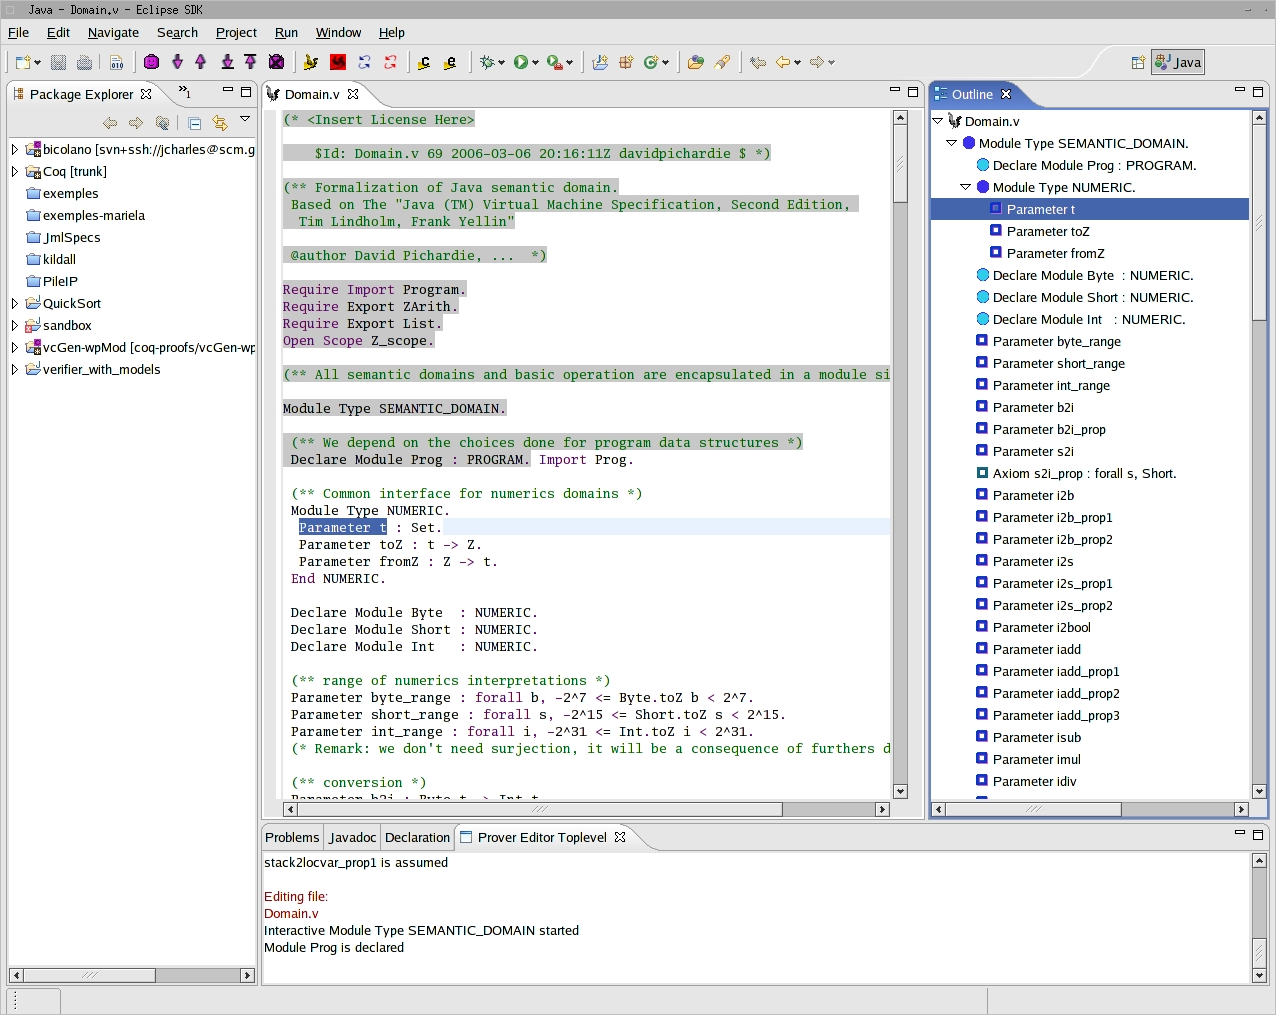
\includegraphics[width=\linewidth]{screenshot1}
\end{center}
  \caption{A normal execution of ProverEditor}
  \label{scrs1}
\end{figure}
The main features are taken from the above extensions descriptions.
ProverEditor is formed of 4 parts 
(\ref{scrs1}): the editor part, the top-level view which is the output 
from the top-level, the outline and the toolbar (as well as the keyboard 
shortcuts to trigger the actions within the toolbar).

The actions associated with the buttons (\ref{tb}) are:
\begin{itemize}
\item spawn a new top-level
\item progress through the proof
\item progress to the end of the proof
\item undo a step
\item undo to the beginning of the file
\item cancel an action
\end{itemize}

These actions are standard and are just like the ones implemented in 
ProofGeneral
or CoqIde. In fact the general organisation of the view for ProverEditor is 
really near the one found in those two tools. One of the the main feature 
it adds is the syntax highlighting of the top-level output. 
So ProverEditor is basically a simplified version of ProofGeneral 
and CoqIde (with less feature like apply a specific tactic).
Instead it relies on a light-weight and easy to extend for 
new provers API integrated in Eclipse.

\begin{figure}
\begin{center}

\includegraphics[width=0.3\linewidth]{toolbar}
\end{center}
  \caption{The toolbar}
  \label{tb}
\end{figure}

%---------------------------------------------------------------------
\subsubsection{Description}
\label{subsubsec:description}

First we will discuss the main features provided by the ProverEditor plugin
(the basic plugin). This plugin provides some low level handling of the target
prover top-level as well as the basic UI bricks to edit a file from the 
prover and highlight its syntax, show an outline of the file and
progress through a proof with it.

The interaction part gives the ability to manage the interactions like sending
through a stream and receiving data from the top-level from its standard output
and error output.
This part of the plugin correspond to a particular package the 
prover.exec package.
This package evolves mainly around the \\
{\tt prover.exec.toplevel.TopLevel} class
which implements the interface {\tt prover.exec.ITopLevel}. 
When the TopLevel class
is instanciated for a specific prover, it calls a prover specific class giving 
it itself as an argument (passed as an instance from the interface
ITopLevel which has more restrictive methods than the TopLevel class.
The interaction with the top-level is bases on a generic call to sendCommand
if a command has to be sent. In a typical sendCommand scenario, the method
{\tt sendCommand(String)} of the TopLevel class is called, 
afterward a prover specific 
{\tt sendCommand(ITopLevel, String)} is called with an instance of the 
TopLevel as a parameter. The method has to call afterward the primitive
{\tt ITopLevel.sendToProver(String)}, manage the output and throw an 
exception of the type AProverException if something has failed.

There is another method used for the same kind of purpose, the
{\tt undo()} command. It has to trigger an undo command to the
top-level. This method call a prover specific  command
which is meant to undo one step whichever context we are in. In most of
the cases it reduces to a call to the {\tt sendCommand(String)} with the 
right parameter.
For instance for Coq depending on the context it will  reduce to 
sending the {\tt Back 1} command {\tt Undo 1}
 (if we are within a proof) or {\tt Abort}
to cancel a proof.\\

%---------------------------------------------------------------------
\subsubsection{Extending ProverEditor with provers}
\label{subsubsec:extend-prov-with}

The key feature in ProverEditor is the easiness to add
some new provers. To add a new prover one must write an Eclipse plugin
in the standard way and after extend 2 extension points. One forcing
to implement 2 classes, one to help handle top-level interactions, and
the other more prover oriented, to implement more gui related things.

The first extension point to extend is {\tt org.eclipse.ui.editors}.
It is the extension point used to add a new file format handling.
The editor to edit the file is provided by ProverEditor it is the class:
{\tt prover.gui.editor.ProverEditor}. One of the problem with Eclipse
is that extension points have to be statically extended. So ProverEditor
cannot extend the Editor dynamically. Otherwise it would have been easy
to remove this prerequisite, like what was done for the PreferencePage,
even though dynamically extending the preference pages isn't either 
really safe.


The second one is one extension point specific to ProverEditor.
The main things it needs to be specified are the 2 classes that the prover
needs to implement.

Then:\\
Extend also the extension point\\
prover.editor.prover\\
and fill up all the asked parameters\\
(the extension must be the same as the editor extension)\\
The specified name must be the name you will call the prover afterward.\\
The translator tag need to be specified a class that extends:\\
prover.plugins.AProverTranslator.\\
The toplevel tag need to be specified a class that extends:\\
prover.plugins.IProverTopLevel.\\

%~~~~~~~~~~~~~~~~~~~~~~~~~~~~~~~~~~~~~~~~~~~~~~~~~~~~~~~~~~~~~~~~~~~~~
%\subsection{component use via Java APIs}


%=====================================================================
\section{Current Plugins}
\label{sec:current-plugins}

We have made right now several plugins:
\begin{itemize}
\item the core plugin, containing all the basic features which was 
described above.
\item the Coq plugin: to handle the interactions with Coq, send parts of a 
file to Coq
and give an outline of the current edited file.
\item the Coq 'Sugar' plugin, which is used to give a proper API for the 
Coq top-level.
It is already used in Jack \cite{Jack-Web} (the Java Applet Correctness Kit) 
an Eclipse plugin to do static program verification on Java programs 
annotated with JML.

\item the PVS plugin which is well... finished?
\end{itemize}

%~~~~~~~~~~~~~~~~~~~~~~~~~~~~~~~~~~~~~~~~~~~~~~~~~~~~~~~~~~~~~~~~~~~~~
\subsection{The Coq plugin}
\label{subsec:coq-plugin}

This plugin is made to do interaction with Coq. The core features
are inside 3 classes. The mandatory plugin class for Eclipse (Eclipse
needs a plugin class in order to consider it has a plugin. This class
is generated automatically by Eclipse. The two other classes are the one
needed to add the extension to ProverEditor: the one used to handle the
top-level and the other one containing mainly the highlighting parts.

There is another part which is less mandatory: the one to handle the outline.
This adds about 10 classes to represents the leafs and nodes of the treeview.
There are 2 kinds of handling: the leaf kind, containing only constructs
like {\tt Definition}, {\tt Parameter} and other single non-imbricated
definitions. There is another kind of construct, the imbricated ones.
In Coq these are the section and the module. These constructs are of
a binary kind, with one to begin them ({\tt Module m.} or {\tt Section s.})
and one to end them ({\tt End m.} or {\tt End s.}).\\

\begin{figure}
\begin{center}
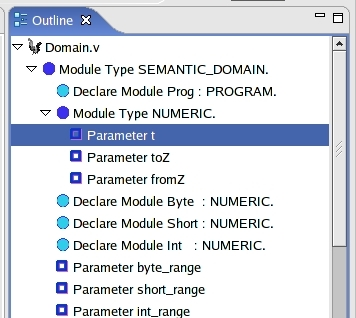
\includegraphics[width=0.5\linewidth]{coqoutline}
\end{center}
  \caption{The outline for Coq}
  \label{outline}
\end{figure}
\begin{figure}
\begin{center}
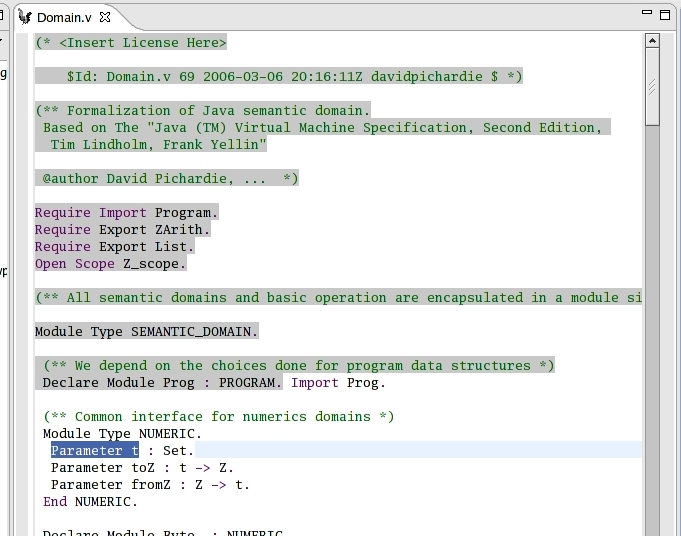
\includegraphics[width=0.6\linewidth]{coqeditor}
\end{center}
  \caption{The editor customized for Coq}
  \label{editor}
\end{figure}

%~~~~~~~~~~~~~~~~~~~~~~~~~~~~~~~~~~~~~~~~~~~~~~~~~~~~~~~~~~~~~~~~~~~~~
\subsection{The Coq sugar-coated plugin}
\label{subsec:coq-sugar-coated}

We have made another plugin which add lots of useless things to the 
basic plugin,
indeed things that can easily be made over the basic implementation.
The purpose of this plugin is only to ease the use of Coq within ProverEditor.

We have mainly added a more complete API to handle Coq. 
It has more high-level 'macros'. 
It subclasses the prover.exec.toplevel.TopLevel to have a real top-level
targeted at Coq. It add some facilities like methods to declare lemmas, 
do a particular standard command or parse the output from Coq to give 
a parsed result of the command instead of the standard output. 
For instance, in Coq there is a command {\tt Show Intros} which
is used to know which variable name Coq would use with its  intros command. 
Here the method gives an array of String with the different variable names.
In Jack we mainly use this API to pretty print the proof obligations with 
Coq in order to have clearer / more user-readable proof obligations.

%~~~~~~~~~~~~~~~~~~~~~~~~~~~~~~~~~~~~~~~~~~~~~~~~~~~~~~~~~~~~~~~~~~~~~
\subsection{The PVS plugin}
\label{subsec:pvs-plugin}

Some intro text. % JRK

%=====================================================================
\section{Conclusion}
\label{sec:conclusion}

We have implemented a lightweight theorem prover within, 
based on the extensions facilities provided by Eclipse. 
To have done it lightweight and minimal in its mandatory
fatures has allowed us to extend it quite fast for the theorem 
provers like Coq or PVS.
What will follow is the extension of these basic features toward more prover 
specific features.
One of the main idea would be to extend it in a component based approach.
Instead of having as in the proof general toolkit one single 
mediator communicating through lighweight protocols to other plugins, 
we will have separated lightweight plugins and their extensions.

%~~~~~~~~~~~~~~~~~~~~~~~~~~~~~~~~~~~~~~~~~~~~~~~~~~~~~~~~~~~~~~~~~~~~~
\subsection{Practical Next Steps}
\label{subsec:practical-next-steps}

The next step will be to have real API plugins for provers. 
It has already begun through Coq's Sugar plugin which only aim 
is to provide this kind of API.
It will be done later on for PVS. Other features that should be added
as separate plugins are the projects and file wizard to creat 
new prover specific files or projects dedicated to a single prover.
Hints like for Java could also be added, like what is done in Eclipse, 
when a variable is pointed its doc or the nearest documentation 
from it should appear. 


%~~~~~~~~~~~~~~~~~~~~~~~~~~~~~~~~~~~~~~~~~~~~~~~~~~~~~~~~~~~~~~~~~~~~~
\subsection{Graphical Representation of Proof Trees}
\label{subsec:graph-repr-proof}

Now we use the outline to get an idea of the file structures for Coq and PVS.
We plan to do an enhanced outline that could give a representation
of the proof tree. This structure more akin of the Proof by Pointing
\cite{bertot94proof}.

% JRK

%~~~~~~~~~~~~~~~~~~~~~~~~~~~~~~~~~~~~~~~~~~~~~~~~~~~~~~~~~~~~~~~~~~~~~
\subsection{Integrating Other Provers}
\label{subsec:integr-other-prov}

We plan to include Isabelle/HOL in a near future.

%~~~~~~~~~~~~~~~~~~~~~~~~~~~~~~~~~~~~~~~~~~~~~~~~~~~~~~~~~~~~~~~~~~~~~
\subsection{Open Research Questions and Challenges}
\label{subsec:open-rese-quest}

Some intro text.

%======================================================================

\bibliographystyle{entcs}
%\bibliography{abbrev,ads,category,complexity,hypertext,icsr,knowledge,languages,linguistics,meta,metrics,misc,modeling,modeltheory,reuse,rewriting,softeng,specification,ssr,technology,theory,web,upcoming,upcoming_conferences,conferences,workshops,verification,escjava,jml,nijmegen}
\bibliography{uitp06}

%======================================================================
% Fin

\end{document}

%%% Local Variables: 
%%% mode: latex
%%% TeX-master: t
%%% End: 
